%%%%%%%%%%%%%%%%%%%%%%%%%%%%%%%%%%%%%%%%%%%%%%%%%%%%%%%%%%%%%%%%%%%%%
% PREAMBLE
%%%%%%%%%%%%%%%%%%%%%%%%%%%%%%%%%%%%%%%%%%%%%%%%%%%%%%%%%%%%%%%%%%%%%
%
% The following two commands will generate a PDF that follows all the 
% requirements for submission and peer review.  Uncomment these commands to 
% generate this output (and comment out the two lines below.)
%
% DOUBLE SPACE VERSION FOR SUBMISSION TO THE AMS
\documentclass[12pt]{article}
\usepackage{ametsoc}
%
% The following two commands will generate a single space, double column paper 
% that closely matches an AMS journal page.  Uncomment these commands to 
% generate this output (and comment out the two lines above. FOR AUTHOR USE 
% ONLY. PAPERS SUBMITTED IN THIS FORMAT WILL BE RETURNED TO THE AUTHOR for 
% submission with the correct formatting.
%
% TWO COLUMN JOURNAL PAGE LAYOUT FOR AUTHOR USE ONLY
%%%%\documentclass[10pt]{article}
%%%%\usepackage{ametsoc2col}
%
%%%%%%%%%%%%%%%%%%%%%%%%%%%%%%%%%%%%%%%%%%%%%%%%%%%%%%%%%%%%%%%%%%%%%
% ABSTRACT
%
% Enter your Abstract here
%%%%%%%%%%%%%%%%%%%%%%%%%%%%%%%%%%%%%%%%%%%%%%%%%%%%%%%%%%%%%%%%%%%%%
\newcommand{\myabstract}{
Direct calculations of the entrainment and detrainment of air into and out of
clouds require a knowledge of the relative velocity difference between the air 
and the cloud surface.  However, a discrete numerical model grid forces the 
distance moved by a cloud surface over a time step to be either zero or the 
width of a model grid cell.  Here we present a method for the subgrid 
interpolation of a cloud surface on a discrete numerical model grid.  This
method is used to calculate entrainment and detrainment rates for an LES model,
which are compared with rates calculated via the direct flux method of 
\cite{Romps2010}.  The comparison shows good agreement between the two methods 
as long as the model clouds are well resolved by the model grid spacing. 
This limitation of our technique is offset by the ability to resolve fluxes 
on much finer temporal and spatial scales, making it suitable for calculating 
entrainment and detrainment profiles for individual clouds.
}
%
\begin{document}
%
%%%%%%%%%%%%%%%%%%%%%%%%%%%%%%%%%%%%%%%%%%%%%%%%%%%%%%%%%%%%%%%%%%%%%
% TITLE
%
% Enter your TITLE here
%%%%%%%%%%%%%%%%%%%%%%%%%%%%%%%%%%%%%%%%%%%%%%%%%%%%%%%%%%%%%%%%%%%%%
\title{\textbf{\large{Interpolation of LES cloud surfaces for use in direct
calculations of entrainment and detrainment}}}
%
% Author names, with corresponding author information. 
% [Update and move the \thanks{...} block as appropriate.]
%
\author{\textsc{Jordan T. Dawe}
	\thanks{\textit{Corresponding author address:} 
	Jordan T. Dawe, 
        Department of Earth and Ocean Sciences, 
        University of British Columbia, 
	6339 Stores Road, 
        Vancouver, BC, 
        V6T 1Z4. 
	\newline{E-mail: jdawe@eos.ubc.ca}}\quad\textsc{and Philip H. Austin}\\
\textit{\footnotesize{Department of Earth and Ocean Sciences, 
                      University of British Columbia, Vancouver, BC}}
}
%
% Formatting done here...Authors should skip over this.  See above for abstract.
\ifthenelse{\boolean{dc}}
{
\twocolumn[
\begin{@twocolumnfalse}
\amstitle

% Start Abstract (Enter your Abstract above.  Do not enter any text here)
\begin{center}
\begin{minipage}{13.0cm}
\begin{abstract}
	\myabstract
	\newline
	\begin{center}
		\rule{38mm}{0.2mm}
	\end{center}
\end{abstract}
\end{minipage}
\end{center}
\end{@twocolumnfalse}
]
}
{
\amstitle
\begin{abstract}
\myabstract
\end{abstract}
}
%%%%%%%%%%%%%%%%%%%%%%%%%%%%%%%%%%%%%%%%%%%%%%%%%%%%%%%%%%%%%%%%%%%%%
% MAIN BODY OF PAPER
%%%%%%%%%%%%%%%%%%%%%%%%%%%%%%%%%%%%%%%%%%%%%%%%%%%%%%%%%%%%%%%%%%%%%

\section{Introduction}

The largest uncertainties in climate sensitivity estimates from Global 
Circulation Model (GCM) simulations come from the subgrid-scale parameterization 
of low clouds \citep{Colman2003,Bony2005,Webb2006}.  Specifically, 
stratocumulus clouds and the transition regime from stratocumulus to trade 
cumulus are the dominant source of variance between models in the estimation of 
the cloud radiative response to changing climate \citep{Williams2009}.

Proper simulation of the subgrid-scale effect of cumulus clouds in GCMs requires 
understanding the rates at which air is entrained into and detrained from the 
clouds. Cloud entrainment and detrainment rates exert influences on profiles of 
cloud properties, the height of the cloud tops, the amount of heat and moisture 
the clouds transport upwards, and the heights at which the clouds deposit that 
heat and moisture.  They also have effects on the vertical transport of 
aerosols out of the boundary layer and the rate at which chemical reactions can 
occur in those aerosols \citep{Barahona2007,Anldrejczuk2008}.

Large Eddy Simulation (LES) is an important tool used in the study of cloud 
entrainment and detrainment. LES models achieve grid resolutions on the order 
of 10-100 m, well within the domain of the Kolmagorov -5/3 turbulence spectrum. 
This allows for a relatively simple turbulence model that captures the 
important statistics of the subgrid-scale eddy fluxes and thus, an accurate 
representation of the atmospheric physics of a domain $\approx$ 10 km$^{2}$, 
which is enough to simulate a field of shallow clouds.  LES can be 
ground-truthed against results taken from field surveys such as the Barbados 
Oceanographic and Meteorological Experiment \citep[BOMEX;][]{Holland1973} or 
the Atmospheric Radiation Measurement \citep[ARM;][]{Brown2002} Program, and 
such comparisons show good agreement between LES and data.

Several recent studies have looked at the life cycle of individual clouds taken 
from LESs, trying to break the cloud field into its component parts 
\citep{Zhao2005,Zhao2005a,Heus2009}.  Estimates of entrainment and detrainment 
rates for individual clouds would be quite useful in these studies, but are 
difficult to achieve. Entrainment and detrainment rates are typically 
calculated in LES by recording budgets of bulk conserved tracer variables, 
such as the total humidity or the liquid water moist static energy, and 
inferring the amount of fluid exchange between cloud and clear air that is 
needed to explain the rate at which that tracer is being vertically advected 
within the cloud field \citep{Siebesma1995}. These budgets typically assume 
the clouds and the cloud environment are horizontally homogeneous slabs; this 
is a much less accurate assumption on the level of an individual cloud, and 
this variability makes bulk tracer calculations on this scale problematic.

Alternatively, entrainment and detrainment could simply be calculated directly 
from the LES velocity, pressure, humidity and temperature fields.  
\cite{Siebesma1998} defines Entrainment and Detrainment as
\begin{equation}
E = -\frac{1}{A}\oint_{\mathbf{\hat{n}}\cdot(\mathbf{u} - \mathbf{u_i}) < 0}
\mathbf{\hat{n}}\cdot(\mathbf{u}-\mathbf{u_i})dl
\end{equation}
\begin{equation}
D = \frac{1}{A}\oint_{\mathbf{\hat{n}}\cdot(\mathbf{u} - \mathbf{u_i}) > 0}
\mathbf{\hat{n}}\cdot(\mathbf{u}-\mathbf{u_i})dl
\end{equation}
where $E$ and $D$ are the entrainment and detrainment rates in kg m$^{-3}$ 
s$^{-1}$, $u$ is the velocity of the air in m s$^{-1}$, $u_i$ is the velocity 
of the cloud surface in m s$^{-1}$, A is the area of the cloud in m,
$\mathbf{\hat{n}}$ is a unit vector directed out the cloud surface, and the 
path integral is taken around the cloud surface at a constant vertical level.
However, the accuracy of this method applied to LES suffers from the need to 
calculate the velocity of the air relative to the cloud surface.  In reality 
these velocities are very nearly identical, \textasciitilde{} 1-2 m s$^{-1}$, 
but the discrete nature of the LES model grid forces the modeled surface 
velocity to be either 0 m s$^{-1}$ or $\Delta x / \Delta t \approx$ 
15-30 m s$^{-1}$, where $\Delta x$ is the model grid spacing and $\Delta t$ 
is the model time step.  The surface of the cloud only moves when a grid 
cell's humidity reaches saturation, and when it does, an entire grid cell 
worth of fluid leaves or enters the cloud.

\cite{Romps2010} recently overcame this problem by averaging the cloud surface 
fluxes over the time needed for an entire grid cell to entrain or detrain.  
The entrainment and detrainment values resulting from this method were 
approximately twice as large as those from previous bulk tracer calculations, 
suggesting bulk tracer calculations contain significant biases.  However, fine 
temporal and spatial resolution of entrainment and detrainment variability is 
difficult to achieve with this method due to the long temporal averages needed.

Here we present a method for calculation of the cloud entrainment and 
detrainment rates that relies on interpolation of the subgrid location of 
the cloud surface.  This method can be used to produce accurate estimates of 
the cloud entrainment and detrainment rates for individual LES clouds.  In 
section 2 we describe this method, in section 3 we describe the 
model configuration we used to test this method, in section 4 we compare this 
calculation with entrainment and detrainment rates calculated using 
\cite{Romps2010} direct flux calculation, and in section 5 we discuss 
our results and present our conclusions.  

%==============================================================================

\section{Method}

Consider a numerical model grid cell containing a cloud surface with normal 
vector $\mathbf{C}$, where $\mathbf{C}$ points outward from the cloud.  This 
surface, combined with $\mathbf{W}$, the portion of the grid cell walls that 
lie within the cloud, encloses a cloud volume $V$ with surface $\mathbf{A}
= \mathbf{C} \cup \mathbf{W}$.  \cite{Siebesma1998} gives the net entrainment 
and detrainment over the cloud surface to be:
\begin{equation}
\label{eq:E_minus_D} 
E - D = \int_C \rho ( \mathbf{u_i} -  \mathbf{u}) \cdot d\mathbf{C},
\end{equation}
where $\rho$ is the air density in kg m$^{-3}$, $\mathbf{u}$ is the velocity
of the air in m s$^{-1}$ and $\mathbf{u_i}$ is the velocity of the cloud 
interface.  Calculating this integral requires knowledge of the velocity field
over the surface of $\mathbf{C}$ and the time evolution of $\mathbf{C}$, 
neither of which is easily calculated in a numerical model.  Instead, we seek a
simplified but equivalent calculation.

To calculate the velocity of the cloud interface, we make use of the Leibnitz 
Theorem:
\begin{equation}
\label{eq:leibnitz} 
\frac{d}{dt}\int_{V(t)} \rho dV = 
  \int_{V(t)} \frac{\partial \rho}{ \partial t} dV 
  + \int_{A(t)} \rho \mathbf{u_i}\cdot d\mathbf{A}.
\end{equation}
Since the walls of the grid cell do not move, $\mathbf{u_i}$ is 0 over 
$\mathbf{W}$.  If we also assume ${\partial \rho}/{ \partial t} \approx 0$, we
get
\begin{equation}
\label{eq:leibnitz2} 
    \rho \frac{d}{dt}\int_{V(t)} dV = 
    \int_{C(t)} \rho \mathbf{u_i}\cdot d\mathbf{C}.
\end{equation}
We then combine equations (\ref{eq:E_minus_D}) and (\ref{eq:leibnitz2}) to give:
\begin{equation}
\label{eq:step1} 
      E - D = \rho \frac{d}{dt}\int_{V(t)} dV
            - \int_C \rho \mathbf{u} \cdot d\mathbf{C}.
\end{equation}

Next we apply the divergence theorem to simplify the flux integral through 
$\mathbf{C}$:
\begin{equation}
\label{eq:divergence} 
\int_{V} \nabla \cdot (\rho \mathbf{u}) dV = 
  \int_{A} \rho \mathbf{u}\cdot d\mathbf{A}
\end{equation}
Due to mass conservation, $\nabla \cdot (\rho \mathbf{u}) = 0$, which implies
\begin{equation}
\label{eq:divergence3} 
  \int_{C} \rho \mathbf{u}\cdot d\mathbf{C} = 
    - \int_{W} \rho \mathbf{u}\cdot d\mathbf{W}
\end{equation}
since $\mathbf{A}$ is the union of $\mathbf{C}$ and $\mathbf{W}$.  Substituting
this into (\ref{eq:step1}) results in
\begin{equation}
\label{eq:entrainment_detrainment} 
E - D = \rho \frac{dV}{dt} + \int_W \rho \mathbf{u} \cdot d\mathbf{W}.
\end{equation}
Therefore, we can find the entrainment and detrainment by calculating the rate 
of change of the cloud volume inside the grid cell and the mass flux through 
the cloudy portion of the grid cell walls.  If equation $E - D$ is greater than 
zero, the total is applied to entrainment and if less than zero, to 
detrainment.  This technique works equally well for flux through any isosurface 
of a scalar quantity defined within the model, though slight modifications must
be made for positive definite quantities.  In this paper we perform these 
calculations for the cloud core, which we define following \cite{Siebesma1995} 
as fluid having condensed liquid water, upward velocity, and positive buoyancy 
relative to the horizontal mean.  

Calculating the mass flux through the grid cell walls can be accomplished using 
the numerical model's advection routine; this is trivial for a model using an 
Arakawa C-grid, while interpolation can give fluxes for other grid 
configurations.  We assume the mass flux is constant over the grid cell wall.  

There are a multitude of interpolation schemes that can be used to determine 
the cloud core volume and cell wall area in a numerical model.  The simplest 
would be to assume that saturated grid cells with positive vertical velocity 
and virtual potential temperature $\theta_v$ (K) greater than the horizontal 
mean are completely filled with cloud core, and otherwise grid cells contain 
no cloud core at all.  We refer to this as the "no interpolation" method.  
Since the cloud core surface only moves when a whole grid cell undergoes 
condensation or evaporation this will result in poor estimates of $dV/dt$ and
$\mathbf{S}$, which will overestimate the entrainment and detrainment.  To 
reduce this overestimate, we interpolate the location of the cloud surface at 
each time step.  Next we describe the interpolation scheme we use for this 
purpose.

%-----------------------------------------------------------------------------

\subsection{Cloud core surface interpolation}

Several standard techniques exist for subgrid isosurface interpolation in the 
field of computer visualization, such as the Marching Cubes algorithm 
\citep{Lorensen1987}.  In the spirit of these techniques, we have implemented 
a scheme that relies on subdividing the grid cells into regular sub-cells, 
finding the location of the cloud surface within these sub-cells, and then 
reassembling the cells to construct the location of the cloud core surface.
Our interpolation scheme, which we refer to as the "tetrahedral interpolation"
method, splits the cubic grid cell into six pyramids, then splits each pyramid 
into eight tetrahedrons (Figure \ref{fig:tetrahedral_scheme}, left 
panel).  This results in forty-eight tetrahedrons, each composed of four 
vertices located at the grid cell center, the center of a grid cell wall, the 
center of a grid cell edge, and a grid cell corner.

Generally, model scalar quantities will be defined on only one of these 
verticies, and so we must interpolate the surrounding grid to determine 
values at the other three points.  On an Arakawa C-grid humidity is defined 
at the grid centers, and so we must interpolate to find the values at three 
of the tetrahedron verticies.  To find values at the center of the grid cell 
wall, we average the two values on opposite sides of the wall; at the grid 
cell edge, we average the four values around the edge; and at the corners, 
we average the values of the eight cells surrounding each corner.

To find the cloud core surface, we must find the location where the total 
humidity equals the saturated humidity, the vertical velocity is zero and 
$\theta_v$ is equal to the horizontal mean of $theta_v$.  First we define a 
variable $q_{diff} = q_t - q_{sat}(T, p)$, where $q_t$ is the total specific 
water content and $q_{sat}(T, p)$ is the saturated specific humidity, all in 
kg water per kg$^{-1}$ of moist air.  $q_{diff}$ is positive for cloudy 
points, negative for clear points, and zero at the cloud surface, representing 
the moisture excess or deficiency relative to the cloud surface.  Similarly, 
we calculate $\Delta \theta_v = \theta_v - \overline{\theta_v}$, where the bar 
represents the horizontal mean, to represent buoyancy excess or deficiency.  
Vertical velocity $w$ requires no new variable to be calculated, but as it is 
defined at the center of the top and bottom of the grid cell, we first 
interpolate $w$ to the center of the grid cell for consistency.

The cloud core surface itself is defined in a similar way to the Marching 
Cubes algorithm \citep{Lorensen1987}.  Each tetrahedron has four vertexes, 
which can either be cloud core or environment, depending on the interpolated 
values of $q_{diff}$, $\Delta \theta_v$, and $w$.  This results in 16 
possible combinations of vertex values that must be considered.  For example,
if the vertexes of a tetrahedron all contain cloud core, the entire 
tetrahedron must contain cloud core, while if three vertexes are core and one 
is environment, the cloud core surface must pass through the tetrahedron.
Many of these cases share symmetries, reducing the number of independent cases 
to four classes.  If the vertexes of a tetrahedron all contain cloud core or 
environment, the surface does not pass through the tetrahedron; this accounts 
for two of the cases.  If only one of the vertexes is clear (or conversely, 
only one is cloudy) than that corner of the tetrahedron is cut by a triangle 
representing the cloud core surface (Figure \ref{fig:tetrahedral_scheme}, 
center panel); this accounts for eight of the cases.  The remaining six cases 
have two vertexes containing cloud core and two vertexes containing 
environment, and result in the tetrahedron being cut by two triangles which 
share a common edge.

The location of the triangles that cut the tetrahedrons are found by 
calculating the fractional distance between connected tetrahedron vertexes at 
which each variable is zero:
\begin{equation}
\label{eq:q_diff_interpolation}
x = \frac{q_{diff}(x_1)}{q_{diff}(x_2) - q_{diff}(x_1)}.
\end{equation}
This calculation is then repeated for $\Delta\theta_v$ and $w$.  The $x$ value 
that returns the smaller cloud core volume is taken to be the location of the 
cloud core surface.   Repeated application of this algorithm to each grid cell 
results in a continuous surface that approximates the subgrid location of the 
cloud core surface (Figure \ref{fig:tetrahedral_scheme}, right panel).

Once the geometry of the case is determined, the area of the cloudy portion of
the model grid cell wall can be calculated by dividing the cloudy area into 
triangles and summing the triangle areas
\begin{equation}
A = \frac{|(\mathbf{b - c}) \times (\mathbf{a - c})|}{2},
\end{equation}
where $\mathbf{a}$, $\mathbf{b}$, $\mathbf{c}$ are the position vectors of the 
vertices of the triangles.  Similarly, the volume of the cut tetrahedron is 
calculated by subdividing it into smaller tetrahedrons, and summing the volumes 
of the sub-tetrahedrons using
\begin{equation}
V = \frac{|\mathbf{a - d} \cdot ((\mathbf{b - d}) \times (\mathbf{c - d}))|}{6},
\end{equation}
where $\mathbf{a}$, $\mathbf{b}$, $\mathbf{c}$, and $\mathbf{d}$ are the 
position vectors of the vertices of the sub-tetrahedrons.  This results in 
all the information needed to measure entrainment and detrainment via equation
(\ref{eq:entrainment_detrainment}).

%==============================================================================

\section{Model Description}

We have implemented both our tetrahedral surface interpolation scheme and the 
time averaging scheme of \cite{Romps2010} in the System for Atmospheric 
Modeling \citep[SAM;][]{Khairoutdinov2003}, allowing the model to calculate 
cloud core entrainment and detrainment via these two methods simultaneously.
We have run these schemes in a standard GCSS Barbados Oceanographic and 
Meteorological Experiment (BOMEX) LES \citep{Holland1973, Siebesma2003}.  
The model was run with a domain extent of 6.4 km x 6.4 km in 
the horizontal and 3.2 km in the vertical.  Model cloud area, vertical 
velocity, and cloud core entrainment diagnosed from bulk conserved tracer 
budgets agree well with the results presented in \cite{Siebesma2003} (not 
shown).

To examine the resolution dependence of our scheme, we ran three models: one at 
25m grid spacing in all directions with a 1.5 second time step, one at 50m grid 
spacing with a 3 second time step, and one at 100m grid spacing with a 6 second 
time step.  For most of the results we present here we rely on the 25m 
resolution model.  The models were each run for 6 hours, and the first 
three hours of simulation were discarded as the model was still adjusting into 
steady-state.  15 minute averages were output for the terms of each of our 
calculations.  Running the 25m resolution model with the tetrahedral surface 
interpolation scheme resulted in a 13\% model slowdown.  

%==============================================================================

\section{Comparison with Romps}

We take the direct entrainment method of \cite{Romps2010}, which we shall 
refer to as the "Romps method", to represent the true entrainment as it uses 
a minimal set of assumptions to perform its calculations.  We therefore use 
the Romps method in this section to evaluate the accuracy of our tetrahedral 
interpolation method.

Comparison of the average values produced by the two methods over three hours 
of model time (Figure \ref{fig:direct_vs_romps}) shows good agreement in the 
vertical profiles of both $E$ and $D$; however, the magnitude of the 
tetrahedral entrainment and detrainment values are slightly higher than the 
Romps value.  This is likely the result of errors in the estimate of the 
velocity of the cloud surface in our tetrahedral scheme, which would tend to 
result in overestimation of the entrainment and detrainment rates.  
However, the tetrahedral scheme is vastly superior to using no interpolation, 
which results in entrainment and detrainment values four times larger than 
the Romps value (not shown).  

There is similar agreement between $\epsilon = E/M$ and $\delta = D/M$, the 
fraction entrainment and detrainment rates, where M is the total vertical 
mass flux within the cloud core in kg m$^{-2}$ s$^{-1}$ and $\epsilon$ and 
$\delta$ have units of m$^{-1}$.  However, large deviations do occur near 
cloud base and top. Some of this deviation results from small differences 
between $E$ and $D$ which are magnified by small values of $M$.  However, at
cloud base and top the Romps method's entrainment is actually larger than the
tetrahedral method's entrainment.  This is due to underestimate of the cloud 
volume by the tetrahedral interpolation in areas where clouds are small; we 
will discuss this underestimate more fully in section 5.  

\subsection{Agreement with the continuity equation}

While $E$ and $D$ are important for calculating changes in cloud properties 
such as temperature and humidity, the vertical profile of cloud fraction is
controlled by their difference, $E-D$.  For comparison with these direct 
flux methods, we also calculate $E-D$ from the continuity equation for a 
turbulent plume: 
\begin{equation}
    \label{eq:continuity}
    \rho \frac{\partial a}{\partial t} 
    + \frac{\partial M}{\partial z}
    = E - D
\end{equation}
To satisfy continuity, the difference between the amount of fluid 
entrained and detrained by the clouds at a given height must equal the 
vertical gradient in cloud mass flux plus the rate in change of the cloud area.
We calculate the vertical gradient of mass flux in equation 
(\ref{eq:continuity}) by interpolating vertical velocities from the edges to 
the center of each grid cell, then averaging total mass flux within the clouds 
using these interpolated velocities.  Fifteen minute average values of mass 
flux were output and the vertical derivative taken via centered differencing.  
Fifteen minute average values of $\partial a/\partial t$ are calculated within 
the model as well.  

Comparison of the tetrahedral values of $E-D$ we have calculated with the
Romps and no interpolation methods shows very close agreement (Figure 
\ref{fig:E_minus_D}).  Of these three calculations, the no interpolation method 
is the most accurate measurement of $E-D$, as we calculate its values directly 
from the model's MPDATA tracer advection routine 
\citep{Smolarkiewicz1990,Khairoutdinov2003} without any modification of the 
cloud surface.  The tetrahedral interpolation method is biased by the method's 
redefinition of the cloud volume, while the Romps method's averaging redefines 
the time at which entrainment and detrainment events take place.  Both these 
schemes result in a more negative $E-D$ value than the no interpolation 
scheme, with the tetrahedral interpolation having slightly less bias.

Our direct flux calculations also agree with the continuity equation fairly 
well (Figure \ref{fig:E_minus_D}), but diverge between cloud base and 1 km 
height.  We take this result to indicate that the interpolation and centered 
differencing we use to calculate mass flux divergence for the continuity 
equation results in a different estimate of mass continuity than the direct 
model fluxes.  Thus suggests the value of $E-D$ is remarkably sensitive to 
the details of the numerical scheme used to calculate the fluxes.  For 
consistency with the underlying model numerics, we recommend these 
calculations be implemented using the same advection scheme used by the 
numerical model in which they are implemented.

%-----------------------------------------------------------------------------

\subsection{Correlation between Romps and Tetrahedral methods}

So far we have shown that our tetrahedral interpolation produces entrainment 
and detrainment values that agree reasonably well with those produced by the 
Romps method.  However, this does not ensure that the same variability is 
displayed by the two calculations.  To analyze the variability, we take the 
correlation of the fifteen-minute averaged $\epsilon$ and $\delta$ values 
calculated via the two methods over the three hour model run at each height 
to generate correlation profiles.  We use $\epsilon = E/M$ and $\delta = D/M$ 
to analyze the variability as $E$ and $D$ are both strongly correlated with 
cloud volume; more cloud volume with the same entrainment velocity results in 
larger entrainment.  Dividing by the mass flux removes this area dependence.
Heights at which the model does not have clouds for the entire three hour 
period are excluded from the calculation.  

Correlations between the Romps and tetrahedral interpolation methods for both 
$\epsilon$ and $\delta$ are significant at the 99\% confidence level over most 
of the cloud layer (Figure \ref{fig:correlations}).  Values near cloud 
base and top show no correlation, which we would expect given the poor 
agreement between the average values of $\epsilon$ and $\delta$ between the 
two methods in these regions (Figure \ref{fig:direct_vs_romps}, d and e).  We
take these results to show general good agreement between our tetrahedral 
interpolation scheme and the time averaging scheme of Romps over relatively 
large time and space averages.  

\subsection{Behavior over different time and space scales}

The Romps method relies on averaging over sufficiently long time scales for 
several grid cells to complete an entrainment or detrainment cycle.  The 
tetrahedral interpolation scheme, on the other hand, has no such limitation.  
For example, the tetrahedral interpolation values horizontally averaged over 
the whole model domain at a given height show little change in variability 
between instantaneous values, 1 minute average values, and 5 minute average 
values (Figure \ref{fig:averaging_convergence}).  The Romps method, on the 
other hand, shows jumps on the order of 50\% of the mean from time step to 
time step.  Over 1 minute averages, the Romps method has variability 
similar to that shown by the tetrahedral interpolation method without any 
averaging, and does not settle down to a stable value until 5 minute averages 
are taken.

When the spatial variability of the two schemes are examined, the Romps 
method shows sparse measurement coverage, even when one minute average values 
are taken (Figure \ref{fig:spatial_variability}).  Tetrahedral interpolation 
values show a relatively smooth spatial distribution at the scale of an 
individual cloud, and tend to be smaller than the Romps method values.  
This is the primary advantage of the tetrahedral interpolation method: it 
allows instantaneous measurements of entrainment and detrainment rates at the 
individual cloud level.

\subsection{Dependence on model resolution}

Both the Romps and tetrahedral methods display relatively strong dependence 
on model resolution, with $E$ and $D$ decreasing as grid resolution becomes 
coarser (Figure \ref{fig:resolution_dependence}).  Furthermore, while $E$ 
and $D$ calculated via the two direct methods show good agreement at 25m 
resolution, the tetrahedral interpolation method systematically 
underestimates the values calculated by the Romps method as grid spacing 
becomes coarser; at 100m resolution, the difference in the values exceeds 
50\%.  Since poor estimation of motion of the cloud surface relative to the 
air should on average result in an over-prediction of $E$ and $D$, a 
different error must be dominating the tetrahedral calculation.

This error is likely related to a systematic underestimate of the cloud volume 
as calculated by the tetrahedral interpolation method when estimating the 
volume of a cloud that occupies a single model grid cell.  Consider such an 
isolated cloud cell, surrounded by clear grid cells in the 2D plane (Figure 
\ref{fig:interpolation_bias}).  For simplicity, instead of considering the 
full cloud core calculation, let us consider simply the condensed water.
Assume the cloud cell has a $q_{diff}$ value of 1 g kg$^{-1}$, and the clear 
cells -1 g kg$^{-1}$.  The Romps calculation, in agreement with the model 
assumptions, will treat this entire grid cell as containing cloud.

The tetrahedral calculation, on the other hand, will underestimate the cloud 
volume.  At the cell edge points, the $q_{diff}$ value will be averaged between
adjacent cells, giving $q_{diff} = 0$ and placing the cloud surface at the grid 
cell wall, exactly as expected.  At the cell corners, however, the four 
surrounding $q_{diff}$ values average to give $q_{diff} = -0.5 g kg^{-1}$, and 
interpolation of this value between the corner and the cell center puts the 
cloud surface at 2/3 the distance between the center and the corner.  This 
effect will occur anytime a single cloud cell is present and multiple clear 
cells are averaged to form interpolation values.

Since the interpolation results in less cloud volume, less entrainment and 
detrainment is measured, since there is less cloud volume with which to 
entrain or detrain.  However, this effect only becomes an issue when a 
significant fraction of the cloud field has a spatial scale on the order of 
the model grid spacing.  This can be seen by comparing vertical profiles of 
the total cloud core fraction for the three model resolutions (Figure 
\ref{fig:area_comparison}).  The 25m grid spacing model tetrahedral 
interpolation volume shows very little underestimate compared to the no 
interpolation cloud core fraction, but the 100m model interpolated volume is 
reduced in size by 50\% of the uninterpolated value.

This underestimate of the volume of isolated cloud cells is an inherent 
feature of surface interpolation, since as a cloud evaporates, the 
interpolated volume would decrease smoothly to zero.  Thus, clouds with a 
volume on the order of the model grid spacing will always have their volume 
underestimated by interpolation.  We have not been able to find a simple way 
to correct for this, as the effect is non-linear and is not corrected simply 
by scaling the entrainment values by the ratio of the interpolated to 
non-interpolated cloud volumes.  Therefore, the tetrahedral interpolation 
method must rely on having sufficient grid resolution to minimize this effect.

%==============================================================================

\section{Discussion and Conclusions}

The good agreement between our technique and the Romps method at fine grid 
spacing gives us confidence that our calculation is a valid representation 
of the flux through the cloud surface.  However, as our method redefines the 
cloud volume, there are interpretation issues when comparing the fluxes 
calculated by the two methods.  For example, consider a cloud that occupies a 
single grid cell.  Assume that over the course of a model time step, the 
liquid water content of the cloudy grid cell decreases, while advective 
processes maintain the moisture in the grid cell's surroundings at a constant 
value.  The Romps calculation will interpret this change as being the result 
of entrainment of environmental air drying the fluid in the grid cell.  Our 
surface interpolation, however, will come to the opposite conclusion: the 
reduction of liquid water content will move the interpolated cloud surface 
closer to the grid cell center, reducing the volume of the cloud and thus 
detraining cloud fluid.  We believe effects like this explain why the 
tetrahedral interpolation method estimates $E$ and $D$ values that are 
smaller than those estimated via the Romps method at coarse grid resolution.

\citet{Romps2010} found that values of direct entrainment and detrainment were 
significantly higher than values calculated via bulk tracer budgets: our 
method supports this conclusion (at least at high enough grid resolution).  
Romps interpreted the smaller tracer budget values to be the result of assuming
all entrainment and detrainment occurs with fluid having the mean properties of
the environment or the cloud core, respectively.  This difference between the 
bulk tracer and direct entrainment calculations suggests that significant 
recirculation occurs around the clouds, with an average air parcel entering 
and leaving the cloud more than once.  

Furthermore, \cite{Brown1999} found entrainment and detrainment calculated via
bulk tracer budgets depended on LES model resolution surprisingly little, in 
contrast to the strong resolution dependence shown by the direct fluxes.
This suggests that changes in this recycling of cloudy air with model 
resolution compensate the mass flux changes resulting in little apparent $E$ 
and $D$ variability in the tracer budgets.  Both these effects suggest an 
understanding of the dynamics of the moistened environment immediately outside 
the clouds may be important for accurate parameterization of cloud property 
exchanges.

We have shown that by interpolating the location of cloud surfaces in an LES
model we have been able to calculate reasonable entrainment and detrainment 
rates directly from model mass fluxes.  These fluxes agree well with the 
direct entrainment method of Romps, with the caveat that the clouds must be 
well resolved by the model grid spacing so as to minimize underestimate of the 
cloud volume by the interpolation scheme.  This tetrahedral interpolation 
scheme gives significant benefits over the Romps method over short time and 
small spatial scales, generating statistically well-behaved results suitable 
for use in examining entrainment and detrainment variability over the life 
cycle of an individual cloud.

Finally, we note that nothing in our technique is dependent on the shallow 
cumulus cloud regime, on indeed on clouds at all; it should be equally useful
in calculating entrainment and detrainment through any material surface in a 
numerical model, subject to the caveats we have mentioned.

%==============================================================================


\begin{acknowledgment}
This paper benefited from helpful discussions with Fleur Couvreux and 
Catherine Rio.  Support was provided by the Canadian Foundation for Climate 
and Atmospheric Science through the Cloud Aerosol Feedback and Climate 
network.  All figures were generated using the matplotlib library in the 
Python programming language.
\end{acknowledgment}

% Use appendix}[A], {appendix}[B], etc. etc. in place of appendix 
% if you have multiple appendixes.
%\ifthenelse{\boolean{dc}}
%{}
%{\clearpage}
%\begin{appendix}
%\section*{\begin{center}Appendix Title Is Entered Here (Primary heading)\end{center}}
%\subsection{First appendix secondary heading}

%\subsection{Second appendix secondary heading}

%\subsubsection{First appendix tertiary heading}

%\subsubsection{Second appendix tertiary heading}

%\paragraph{First appendix quaternary heading}

%\paragraph{Second appendix quaternary heading}

%\end{appendix}

% Create a bibliography directory and place your .bib file there.
\ifthenelse{\boolean{dc}}
{}
{\clearpage}
\bibliographystyle{./ametsoc}
\bibliography{./bibliography/entrainment_interpolation}

%%%%%%%%%%%%%%%%%%%%%%%%%%%%%%%%%%%%%%%%%%%%%%%%%%%%%%%%%%%%%%%%%%%%%
% FIGURES
%%%%%%%%%%%%%%%%%%%%%%%%%%%%%%%%%%%%%%%%%%%%%%%%%%%%%%%%%%%%%%%%%%%%%

\begin{figure}[t]
  \noindent
  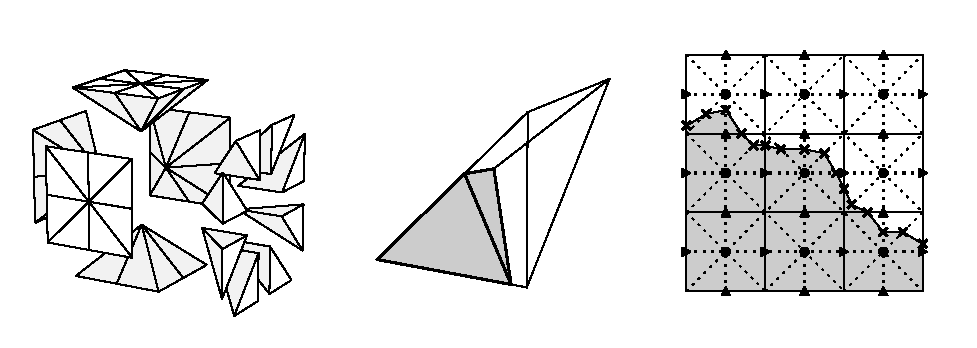
\includegraphics[width=40pc,angle=0]{./figures/tetrahedral_scheme}\\
  \caption{Schematic representation of the tetrahedral interpolation 
  method.  Left panel shows the subdivision of the model grid cell into 
  forty-eight tetrahedrons.  Center panel shows the interpolation of the cloud 
  surface within a sub-tetrahedron between points at the four vertices of the 
  tetrahedron.  Right panel shows a horizontal slice through the model's 
  Arakawa C-grid.  Rightward pointing triangles represent u-velocity points, 
  upward pointing triangles represent v-velocity points, circles represent 
  bulk tracer quantities such as temperature or humidity, and x represents 
  the location of the cloud surface interpolation points.  Dotted lines show 
  the boundaries of the tetrahedral subdivision of the grid, and grey shading 
  represents cloud volume.}
  \label{fig:tetrahedral_scheme}
\end{figure}

\begin{figure}[t]
  \noindent
  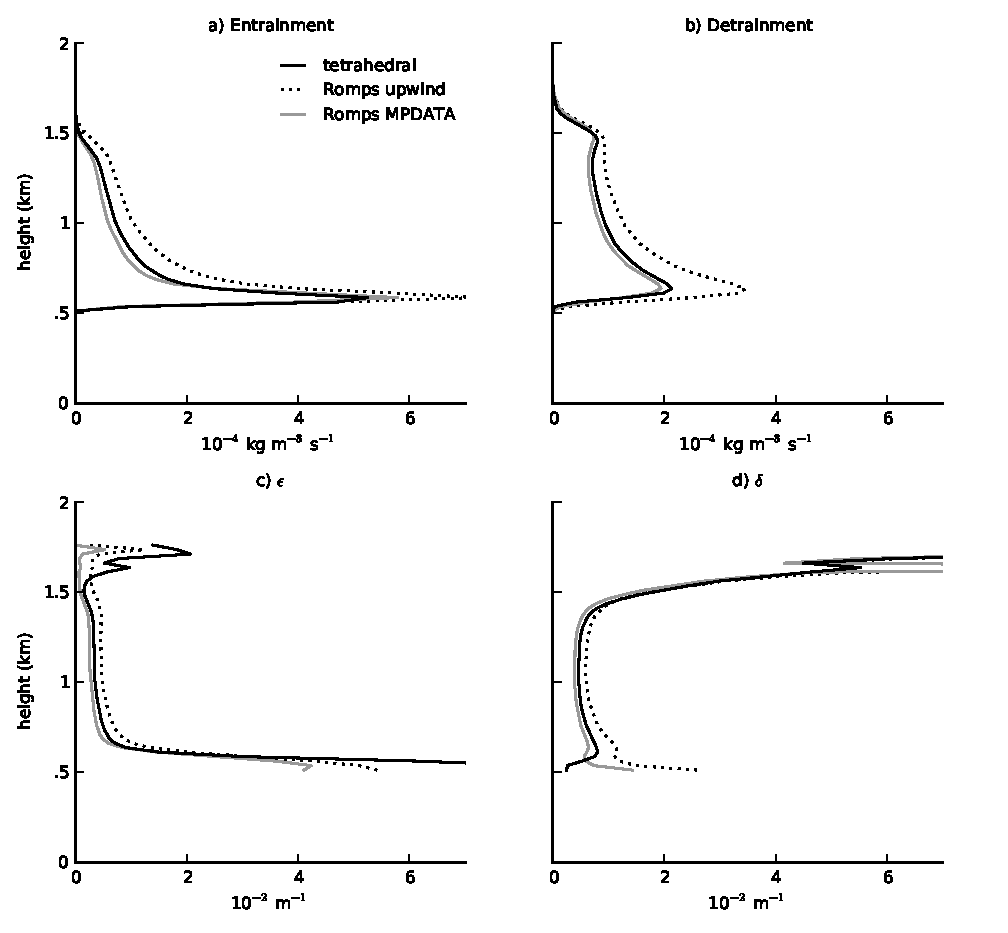
\includegraphics[width=40pc,angle=0]{./figures/direct_vs_romps}\\
  \caption{Comparison of mean model profiles of core a) entrainment and b) 
  detrainment calculated using the Romps method (grey line) and the
  tetrahedral interpolation method (black line).  c) Ratio of Romps 
  method to tetrahedral interpolation method rates of entrainment 
  (black) and detrainment (grey).  d) and e) are the same as a) and b) but 
  for the fractional entrainment and detrainment rates.}
  \label{fig:direct_vs_romps}
\end{figure}

\begin{figure}[t]
  \noindent
  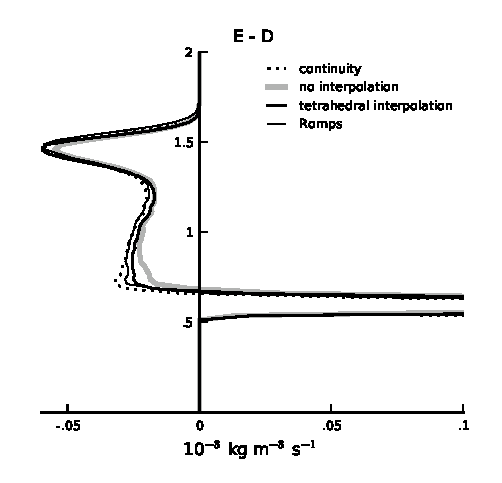
\includegraphics[width=19pc,angle=0]{./figures/E_minus_D}\\
  \caption{Average profiles of entrainment minus detrainment calculated using 
  the continuity equation (dotted line), direct fluxes with no surface 
  interpolation (grey line), the tetrahedral interpolation method
  (thick black line), and the Romps method (thin black line).
  }\label{fig:E_minus_D}
\end{figure}

\begin{figure}[t]
  \noindent
  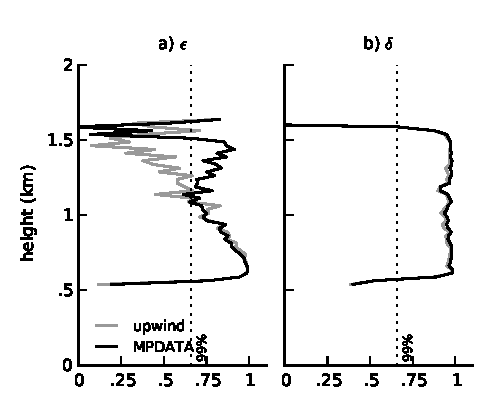
\includegraphics[width=19pc,angle=0]{./figures/correlations}\\
  \caption{
  Profiles of the correlation between the Romps method and the
  tetrahedral interpolation method for a) entrainment and b) detrainment.  
  Dotted line shows the 99\% confidence level for a significant correlation.
  }
  \label{fig:correlations}
\end{figure}

\begin{figure}[t]
  \noindent
  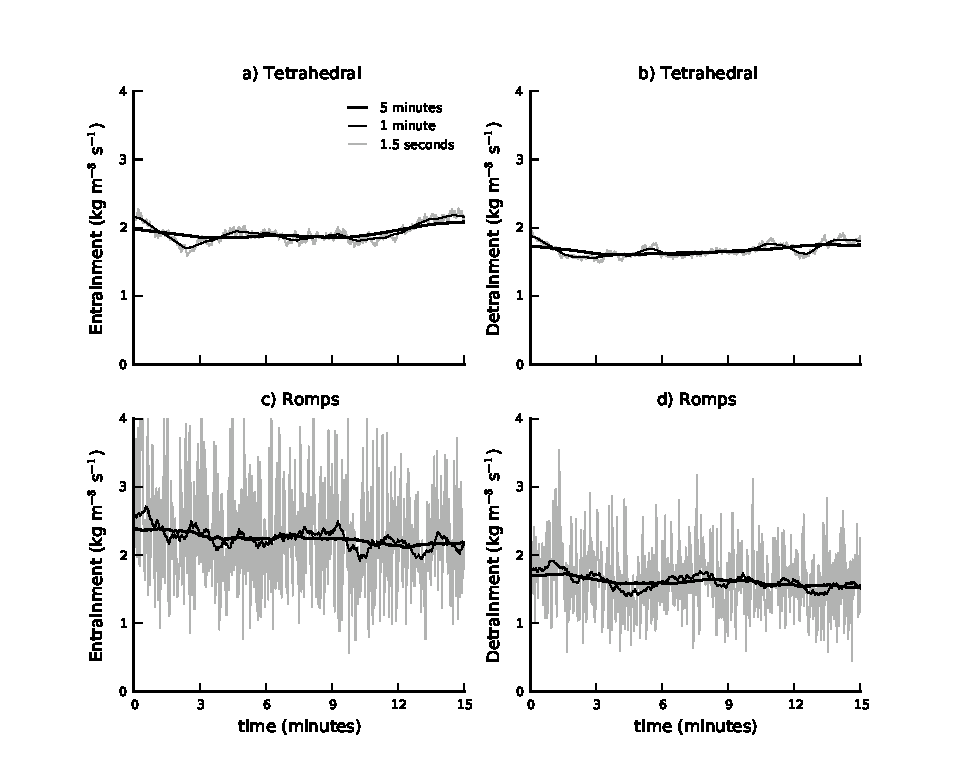
\includegraphics[width=39pc,angle=0]{./figures/averaging_convergence}\\ 
  \caption{Time variability of entrainment and detrainment horizontally 
  averaged over the model domain at a height of one kilometer calculated via 
  a) the tetrahedral interpolation method and b) the Romps method.
  }
  \label{fig:averaging_convergence}
\end{figure}

\begin{figure}[t]
  \noindent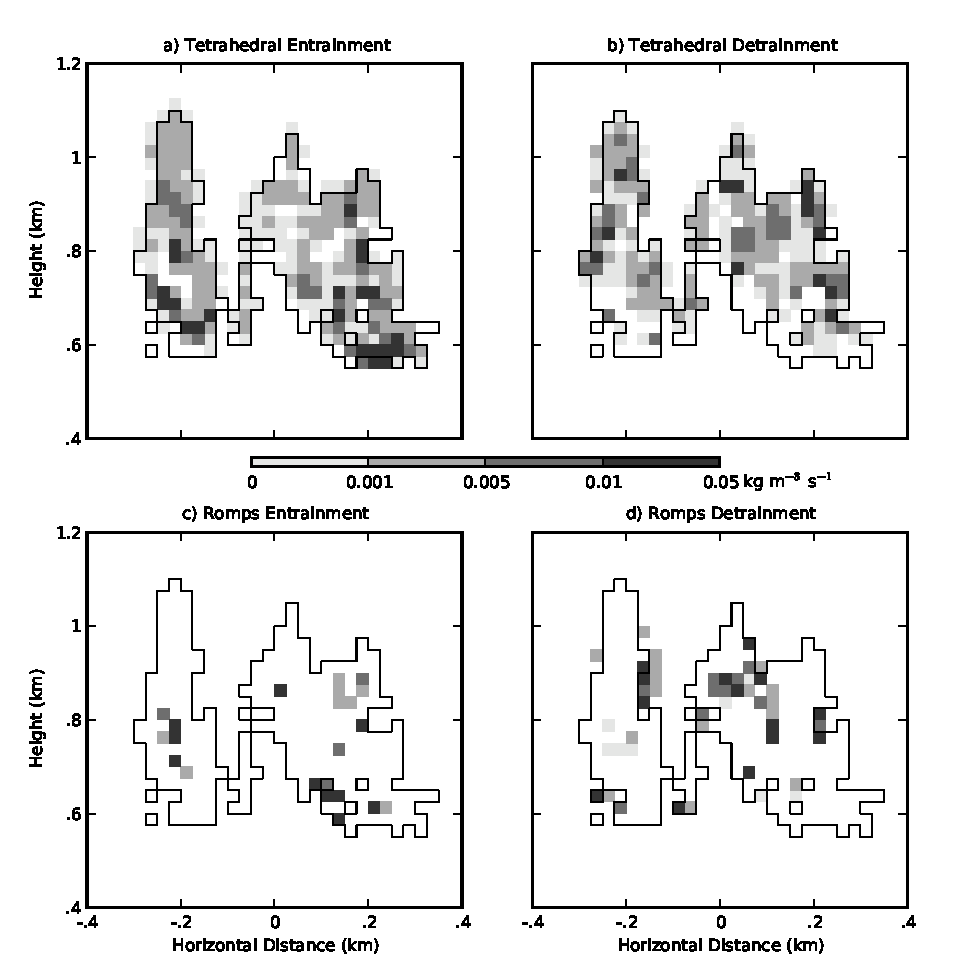
\includegraphics[width=39pc,angle=0]{./figures/spatial_variability_1min}\\ 
  \caption{Vertical cross-section of a model cloud showing one minute averaged 
  entrainment (a, c) and detrainment (b, d) calculated using the tetrahedral 
  interpolation method (a, b) and the Romps method (c, d).  Greyscale indicates 
  amount of entrainment or detrainment, lines show the region where condensed 
  liquid water exists.
  }
  \label{fig:spatial_variability}
\end{figure}

\begin{figure}[t]
  \noindent
  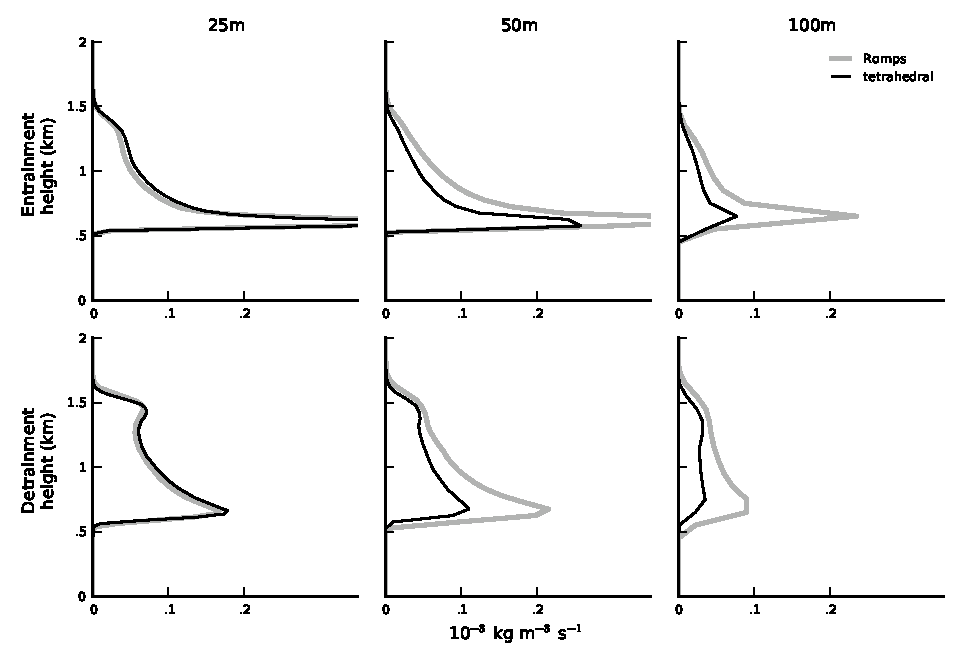
\includegraphics[width=39pc,angle=0]{./figures/resolution_dependence}\\
  \caption{Mean entrainment (top row) and detrainment (bottom row) calculated
  at 25m (left column), 50m (center column), and 100m (right column) grid 
  spacing using the Romps method (grey line) and the tetrahedral 
  interpolation method (black line).
  }
  \label{fig:resolution_dependence}
\end{figure}

\begin{figure}[t]
  \noindent
  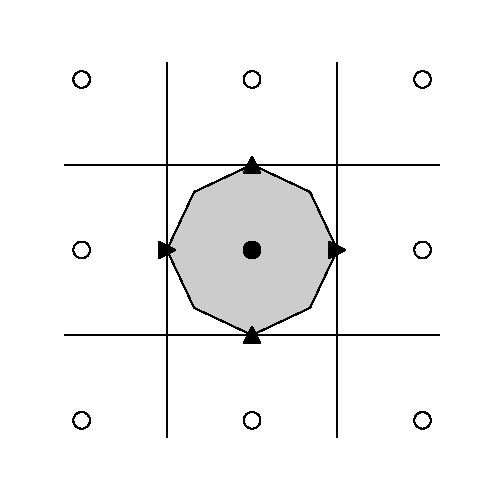
\includegraphics[width=19pc,angle=0]{./figures/interpolation_bias}\\ 
  \caption{Schematic showing bias in the tetrahedral interpolation method 
  which leads to underestimation of cloud volume.  Rightward pointing 
  triangles represent u-velocity points, upward pointing triangles represent 
  v-velocity points, and circles represent bulk tracer quantity points.
  Black circles indicate cloudy points with total specific water 1 g 
  kg$^{-1}$ above the saturated specific humidity, white circle indicate 
  clear points with total specific water 1 g kg$^{-1}$ below the 
  saturated specific humidity.  Grey area indicates the resulting tetrahedral
  interpolation cloud surface.
  }
  \label{fig:interpolation_bias}
\end{figure}

\begin{figure}[t]
  \noindent
  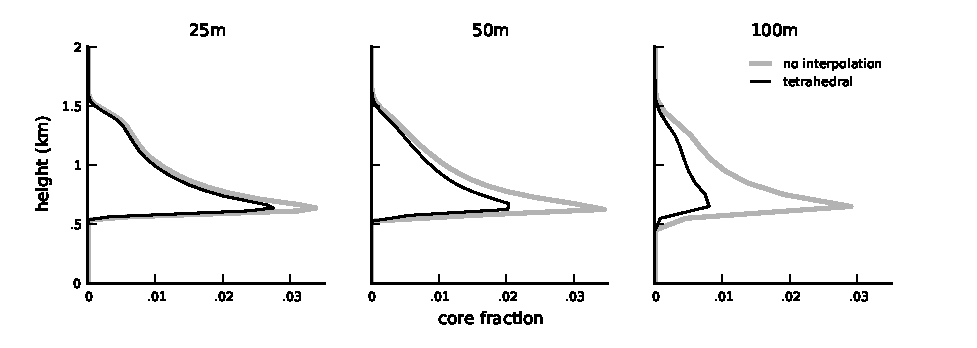
\includegraphics[width=40pc,angle=0]{./figures/area_comparison}\\ 
  \caption{Profiles of cloud core fraction calculated without interpolation 
  (grey line) and with tetrahedral interpolation (black line) at 25m, 50m, 
  and 100m grid spacings.
  }
  \label{fig:area_comparison}
\end{figure}

\end{document}
